\documentclass{article}

% Adopted from the Overleaf Arxiv template

\usepackage{arxiv}

\usepackage[utf8]{inputenc} % allow utf-8 input
\usepackage[T1]{fontenc}    % use 8-bit T1 fonts
\usepackage{hyperref}       % hyperlinks
\usepackage{url}            % simple URL typesetting
\usepackage{booktabs}       % professional-quality tables
\usepackage{amsfonts}       % blackboard math symbols
\usepackage{nicefrac}       % compact symbols for 1/2, etc.
\usepackage{microtype}      % microtypography
\usepackage{lipsum}
\usepackage{graphicx}
\usepackage{multirow}
%\usepackage{booktabs}
\graphicspath{ {./images/} }


\title{Analysis of Five of J.S. Fletcher's Murder Mystery Novels}


\author{
 Jerry Duncan, Everett Rush, Daniel Schultz, and Quan Zhou\\
  Electrical Engineering and Computer Science (EECS)\\
  The University of Tennessee\\
  Knoxville, TN 37996 \\
  \texttt{jdunca51@vols.utk.edu, erush3@vols.utk.edu, dschult9@vols.utk.edu, qzhou10@vols.utk.edu} \\
  }

\begin{document}
\maketitle
\begin{abstract}
  Natural Language Processing is one of the largest and fastest growing Machine Learning fields. Its applicability to such a large variety of problems, makes it both versatile and often used to solve any problem relating to text data. In this work we use very simplistic Natural Language Processing to analyze the plot structure of five different murder mystery books written by J.S. Fletcher. We use Beautiful Soup to scrape the books off of Project Gutenberg, split the books into chapters and sentences using Regular Expressions, and then search through the corpora for answers to six plot-defining questions. From these we create a good view of how each novel's plot structure relates to each other.
\end{abstract}


\keywords{Natural Language Processing \and Plot Structure Analysis \and Regular Expressions}


\section{Introduction}

Machine learning techniques have been applied in many scientific domains such as healthcare, biology, chemistry, phsyics, etc. Other fields such as humanities have a unique set of challenges and a much fewer applications. One such challenge is that everyone has their own opinion about the quality and interpretation of a work. Some people may enjoy and highly praise one work while others may not. Furthermore, because art is made for humans, art usually invokes a human reaction or emotion. For example, an author may add an element of suspense into a work of fiction or have a comic moment. These qualities can be difficult to describe to other humans, let alone a computer. \\

Plot structure analysis is a task that does not immediately translate well to a machine learning problem. Plot structure analysis plots the main sequences of events in a work of fiction on a timeline. Often the context surrounding these main events is described as well. Writers and critics usually perform this task by hand as they analyze a work of fiction. Plots often contain surprises and twists that catch readers off-guard. Characters often change and evolve throughout the course of a novel as well. For example a friendly character could turn into a criminal or the least suspecting person could have committed the gravest of crimes. \\

In this work we perform a computational analysis of the plot structure of five J.S. Fletcher novels. Each novel contains a detective that goes about solving a crime or supposed crime. Many times, the detective is not a detective by trade but gets dragged into an investigation due to circumstances. The novels always end by tying up all the loose ends and solving the crime. Often times, some unexpected events happen along the way such as the suicide of the lead character. \\

\section{Approach}
\paragraph{Data Sources} We selected five murder mysteries by J.S. Fletcher for analysis: Dead Men's Money \cite{deadmen}, The Middle of Things \cite{middleofthings}, The Middle Temple Murder \cite{middletemplemurder}, The Talleyrand Maxim \cite{tallyrandmaxim}, and Scarhaven Keep \cite{scarhavenkeep}. His works are freely available through Project Gutenberg \cite{gutenberg}.  We selected these five murder mysteries because of their conformity to standard literary tropes and their potential to reveal hidden structure in Fletcher's works. In each book, there is always an investigator, a murderer(s), and a timeline from the discovery of a murder to the identification of the murderer(s). However, this does not imply that they all have the same, overly rigid structure, as we found that some of the novels contain complex subplots. For instance, a killer might have multiple pseudonyms, receive assistance from a number of co-conspirators, or be revealed to not be a murderer at all. Very often the murder is enacted to support a larger objective such as the concealment of a second will that removes the killer from receiving their inheritance.

\paragraph{Data Preparation} For The Tallyrand Maxim specifically, we used the Stanford Core NLP Part-of-Speech (POS) tagger from the Natural Language TookKit (NLTK) to help identify instances where the term \textit{will} is used as a noun rather than a verb, to prevent false positives that do not refer to the murderer's goal. We also used a Wordnet synonym set to identify synonyms of \textit{murder} and \textit{will}, all of which were manually transformed into their respective lemmas.

To help split the chapters into sentences that we could further analyze, we used a complex, handcrafted regex expression to split sentences that is better described in Appendix \ref{sect:regex}. We also used NLTK to both identify proper nouns and to split contractions with its Treebank Word Tokenizer. 

\paragraph{Background Research} We conducted extensive background research to identify the investigator, criminals, and other potential accomplices. This was a manual process because there are no in-depth plot summaries or analyses for any of the J.S. Fletcher works. GoodReads \cite{goodreads} contains the most basic summaries of many books. Kadaxis \cite{kadaxis} has a good list of characters. We had to read large portions of the books because our resources were lacking a list of the criminals, the ending, and the other suspects. \\

\paragraph{Analysis} We started by performing regex searches for the first occurrence of when the principle characters appeared in their respective novels, as well as every co-occurrence of the investigator and murderer(s). We also recorded the number of times that \textit{murder} and \textit{will} occurred in The Tallyrand Maxim. And, as noted in \textbf{Data Preparation}, we filtered \textit{will} by part of speech to remove instances where it was used as a verb.

\section{Results}
After extensive investigation of deep reading and manual regex search, the detailed information of the above five Fletcher's novels is shown from Table 1 to Table 5.

Furthermore, using the Regex approach to search corresponding detective, perpetrator and suspects, the results are shown in table 6. And question 1 to question 6 are denoted as 1-6. Below illustrates question 1-6 that we answered for each book.
\begin{enumerate}
\item When does the detective (or a pair) occur for the first time - chapter \#, the sentence(s) \# in a chapter;
\item When is the crime first mentioned - the type of the crime and the details - chapter \#, the sentence(s) \# in a chapter;
\item When is the perpetrator first mentioned - chapter \#, the sentence(s) \# in a chapter;
\item What are the 3 words that occur around the perpetrator on each mention (i.e., the three words preceding, and the three words following the mention of a perpetrator);
\item When and how the detective/detectives and the perpetrators co-occur - chapter \#, the sentence(s) \# in a chapter;
\item When are other suspects first introduced - chapter \#, the sentence(s) \# in a chapter.
\end{enumerate}

Based on our analysis, we obtained the following results: \\
\\

\subsection{The Middle of Things}
\textbf{Total Chapters}: 29 \\
\begin{enumerate}
    \item Detective Viner is first referenced in chapter 1 sentence 1. \\
    \item Perpetrator Cortelyon first referenced chapter 2 sentence 54. The text reads, "Cortelyon saw that by killing Ashton he alone would have the secret; he evidently got two accomplices who were necessary to him." \\
    \item The crime of murder first appears in chapter 1 sentence 76. The text reads, "Then he saw white linen, and a bloodstain slowly spreading over its glossy surface." \\
    \item There are 90 context words total. See Table \ref{tab:tmot} \\
    \begin{table}[]
        \centering
        \begin{tabular}{c|c|c}
        word & context word & count \\ \hline
Cortelyon & Dr & 10 \\
Cortelyon & Ashton & 5 \\
Cortelyon & hed & 3 \\
Cortelyon & asked & 2 \\
Cortelyon & square & 2 \\
Cortelyon & years & 2 \\
Cortelyon & Cave & 2 \\
Cortelyon & wed & 2 \\
Cortelyon & papers & 2 \\
Cortelyon & found & 2 \\
        \end{tabular}
        \caption{Caption}
        \label{tab:tmot}
    \end{table}
    \item Detective-perp cooccurrences in (chapter, sentence) form: [(3, 78), (28, 134)] \\
    \item Other Suspects Penkridge first referenced chapter 1 sentence 1 \\
\end{enumerate}

\subsection{Scarhaven Keep}
\textbf{Total Chapters}: 31 \\
\begin{enumerate}
    \item Detective Richard Copplestone first referenced chapter 1 sentence 39 \\
    \item There are a series of perpetrators. Addie Chatfield and her husband impersonate a rich person. With the help of her father, Peter, they steal the Greyle's family weath. They are first referenced in chapter 4 sentence 114. \\
    \item There is a plot twist introduced in the last chapter. Originally they are investigating the murder of Basset Oliver. This turns out to be an accident not murder. You then find out the real crime is stealing money. \\
    \item The number of context words is 969. See Table \ref{tab:scar} \\
    \begin{table}[]
        \centering
        \begin{tabular}{c|c|c}
        word & context word & count \\ \hline
Chatfield & Mr & 74 \\
Chatfield & Peter & 46 \\
Chatfield & said & 34 \\
Chatfield & Addie & 30 \\
Chatfield & Miss & 30 \\
Addie & Chatfield & 30 \\
Chatfield & I & 26 \\
Chatfield & Vickers & 26 \\
Peter & Chatfield & 23 \\
Chatfield & know & 18 \\
Chatfield & replied & 16 \\
        \end{tabular}
        \caption{Caption}
        \label{tab:scar}
    \end{table}
    \item Detective-perp cooccurrences in (chapter, sentence) form: [(6, 3), (6, 32), (8, 161), (18, 73), (21, 47), (21, 84), (21, 98), (22, 87), (23, 45), (27, 37), (29, 110), (30, 189), (31, 1), (31, 78), (31, 160)] \\
    \item Audrey Greyle is a suspect at first. She is introduced chapter 3 sentence 166. \\
\end{enumerate}


\subsection{The Talleyrand Maxim}
\textbf{Total Chapters}: 28 \\
\begin{enumerate}
    \item Detective Linford Pratt first referenced chapter 1 sentence 1. \\
    \item The perpetrator Harper Mallathorpe is first referenced chapter 1 sentence 57. \\
    \item Crime murder first referenced chapter 7 sentence 93. There is a plot twist in the last chapter. Initially they investigate a murder, but it turns out the man left town and went to America. The real crime is that Harper destroyed her husband's will because he left his money to a charity. You can see this plot twist visually by inspecting Figure \ref{fig:The Talleyrand Maxim}. John Mallathrope's will is introduced early on as the murder is investigated. Then he leave it alone for a few chapters. Fletcher reintroduces it again a few chapters before the end. Then in the last chapter the plot twist occurs, and he ties it all together.\\
    \item The number of context words is 635. See Table \ref{tab:talleyrand}.
        \begin{table}[]
        \centering
        \begin{tabular}{c|c|c}
        word & context word & count \\ \hline
Mallathorpe & Mrs & 388 \\
Mallathorpe & Miss & 104 \\
Mallathorpe & John & 80 \\
Mallathorpe & Nesta & 60 \\
Mallathorpe & Mr & 56 \\
Mallathorpe & I & 48 \\
Mallathorpe & Pratt & 44 \\
Mallathorpe & said & 40 \\
Mallathorpe & Harper & 30 \\
Harper & Mallathorpe & 30 \\
Mallathorpe & see & 28 \\
Mallathorpe & know & 28 \\
Mallathorpe & would & 18 \\
Mallathorpe & Eldrick & 18 \\
Mallathorpe & time & 16 \\
Mallathorpe & Normandale & 16 \\
Mallathorpe & letter & 16 \\
Mallathorpe & called & 16 \\
Mallathorpe & went & 16 \\
Mallathorpe & doesnt & 16 \\
Mallathorpe & late & 14 \\
Mallathorpe & family & 14 \\
Mallathorpe & But & 14 \\
Mallathorpe & business & 14 \\
Mallathorpe & mother & 14 \\
Mallathorpe & left & 12 \\
Mallathorpe & property & 12 \\
Mallathorpe & died & 12 \\
        \end{tabular}
        \caption{Caption}
        \label{tab:talleyrand}
    \end{table}
    \item Detective-perp cooccurrences in (chapter, sentence) form: [(2, 130), (2, 147), (2, 148), (2, 149), (2, 150), (5, 1), (5, 18), (5, 21), (5, 26), (5, 27), (5, 30), (5, 114), (5, 117), (5, 158), (5, 171), (5, 193), (6, 121), (7, 122), (8, 1), (8, 11), (8, 21), (8, 24), (8, 35), (8, 50), (8, 97), (8, 165), (10, 90), (10, 164), (10, 182), (11, 40), (11, 74), (12, 168), (12, 179), (12, 217), (12, 219), (12, 253), (12, 270), (12, 278), (12, 291), (12, 299), (12, 300), (12, 315), (13, 32), (13, 34), (13, 68), (13, 85), (13, 93), (13, 106), (13, 114), (13, 115), (13, 130), (14, 46), (14, 154), (15, 129), (16, 113), (16, 138), (16, 156), (16, 173), (16, 178), (17, 51), (17, 56), (17, 67), (18, 148), (18, 150), (21, 10), (21, 13), (21, 70), (21, 125), (21, 154), (22, 1), (25, 34), (25, 40), (27, 48), (27, 50), (27, 63)]  \\
    \item Other Suspects Nesta first referenced chapter 2 sentence 17.
\end{enumerate}

\begin{figure}[htbp] 
			\centering 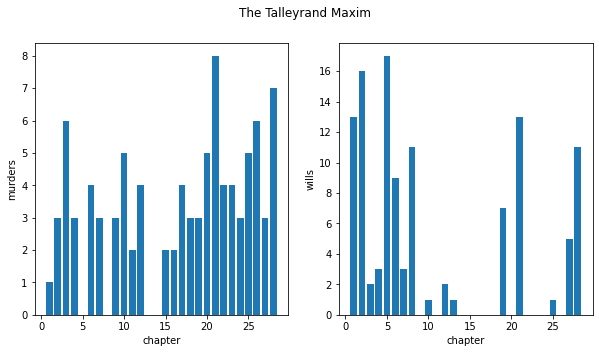
\includegraphics[width=0.65\columnwidth]{images/talleyrandmaxim.png}
			\caption{
				\label{fig:The Talleyrand Maxim} 
				The Talleyrand Maxim
				%\cite{}
			}
\end{figure}

\subsection{The Middle Temple Murder}
\textbf{Total Chapters}: 36 \\

\begin{enumerate}
    \item Detective Frank Spargo is first referenced in chapter 1 sentence 1. \\
    \item Perpetrator Jane Baylis first referenced chapter 19 sentence 24.\\
    \item The crime of murder first appears in referenced chapter 1 sentence 24. \\
    \item There are 360 context words total. See Table \ref{tab:mtm} \\
    \begin{table}[]
        \centering
        \begin{tabular}{c|c|c}
        word & context word & count \\ \hline
        Baylis & Miss & 96 \\
Baylis & Jane & 24 \\
Baylis & But & 14 \\
Baylis & Spargo & 14 \\
Jane & Baylis & 12 \\
Baylis & see & 8 \\
Baylis & said & 8 \\
Baylis & I & 8 \\
Baylis & told & 8 \\
Baylis & looked & 6 \\
Baylis & scornful & 6 \\
Baylis & suddenly & 6 \\
Baylis & came & 6 \\
        \end{tabular}
        \caption{Caption}
        \label{tab:mtm}
    \end{table}
    \item Detective-perp cooccurrences in (chapter, sentence) form: [(19, 41), (21, 153), (23, 11), (23, 13), (23, 34), (23, 35), (24, 1), (24, 22), (25, 17), (26, 31), (27, 6), (27, 8), (27, 17), (27, 59), (29, 71), (30, 133), (36, 131)] \\
    \item Other Suspects Chamberlayne first referenced chapter 6 sentence 156. \\
\end{enumerate}



\subsection{Dead Men's Money}
\textbf{Total Chapters}: 37 \\

\begin{enumerate}
    \item Detective Hugh Moneylaw is first referenced in chapter 1 sentence 19. \\
    \item Perpetrator Gilbert Carstairs first referenced chapter 7 sentence 6.\\
    \item The crime of murder first appears in referenced chapter 1 sentence 3. \\
    \item There are 676 context words total. See Table \ref{tab:dmm} \\
    \begin{table}[]
        \centering
        \begin{tabular}{c|c|c}
        word & context word & count \\ \hline
        Gilbert & Sir & 156 \\
Gilbert & Carstairs & 91 \\
Carstairs & Gilbert & 91 \\
Carstairs & Sir & 84 \\
Gilbert & I & 30 \\
Carstairs & Michael & 27 \\
Carstairs & Lady & 15 \\
Carstairs & Mr & 14 \\
Gilbert & Mr & 12 \\
Carstairs & I & 12 \\
Gilbert & man & 11 \\
Carstairs & yacht & 8 \\
Carstairs & Carstairs & 8 \\
Gilbert & Hathercleugh & 7 \\
        \end{tabular}
        \caption{Caption}
        \label{tab:dmm}
    \end{table}
    \item Detective-perp cooccurrences in (chapter,sentence) form: [(22, 67)] \\
    \item Dead Men's Money has no Other Suspects. \\
\end{enumerate}



%\begin{figure}[htbp] 
%			\centering %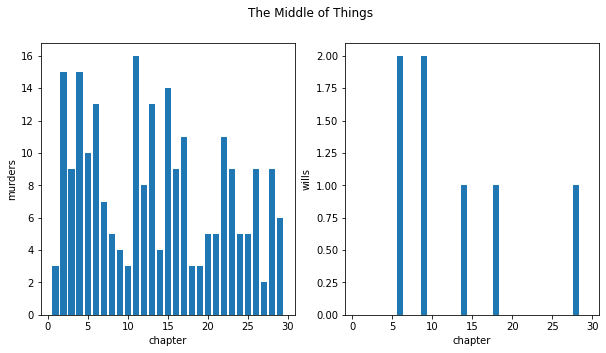
\includegraphics[width=0.65\columnwidth]{images/middlethings.png}
%			\caption{
%				\label{fig:The Middle of Things} 
%				The Middle of Things
%				%\cite{}
%			}
%\end{figure}
%\begin{figure}[htbp] 
%			\centering %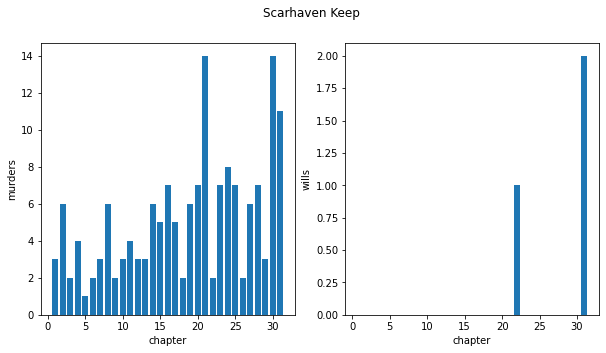
\includegraphics[width=0.65\columnwidth]{images/scarhavenkeep.png}
%			\caption{
%				\label{fig:Scarhaven Keep} 
%				Scarhaven Keep
%				%\cite{}
%			}
%\end{figure}
%\begin{figure}[htbp] 
%			\centering %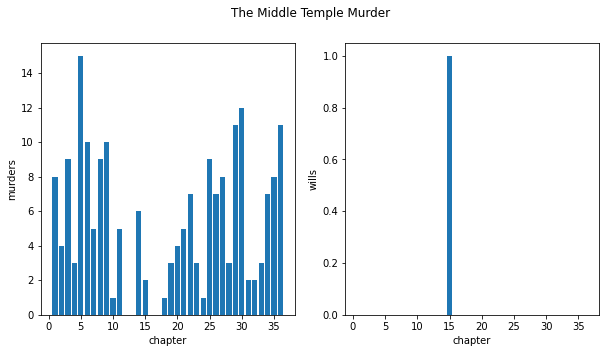
\includegraphics[width=0.65\columnwidth]{images/middlemurder.png}
%			\caption{
%				\label{fig:The Middle Temple Murder} 
%				The Middle Temple Murder
%				%\cite{}
%			}
%\end{figure}


%\begin{figure}[htbp] 
%			\centering %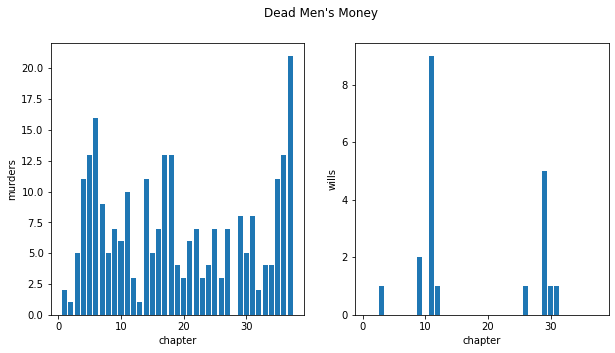
\includegraphics[width=0.65\columnwidth]{images/deadmoney.png}
%			\caption{
%				\label{fig:Dead Men’s Money} 
%				Dead Men’s Money
%				%\cite{}
%			}
%\end{figure}




% Please add the following required packages to your document preamble:
% \usepackage{booktabs}
% \usepackage{multirow}
\begin{table}[htbp]
\centering
\caption{Information of "The Middle of Things"}
\begin{tabular}{@{}l|l|l@{}}
\toprule
\multirow{6}{*}{The Middle of Things} & Detective      & 'Viner'                                                                                                                                                                                                                                                                                                                                                                                                                                                                                                                                                        \\ \cmidrule(l){2-3} 
                                      & Perpetrator    & 'Cortelyon'                                                                                                                                                                                                                                                                                                                                                                                                                                                                                                                                                    \\ \cmidrule(l){2-3} 
                                      & Crime          & 'murder'                                                                                                                                                                                                                                                                                                                                                                                                                                                                                                                                                       \\ \cmidrule(l){2-3} 
                                      & Other Suspects & 'Penkridge'                                                                                                                                                                                                                                                                                                                                                                                                                                                                                                                                                    \\ \cmidrule(l){2-3} 
                                      & Victims        & 'Richard Ashton'                                                                                                                                                                                                                                                                                                                                                                                                                                                                                                                                               \\ \cmidrule(l){2-3} 
                                      & Characters     & \begin{tabular}[c]{@{}l@{}}'Viner', 'Pawle','Ashton', 'Carless','Wickham','Hyde','Marketstoke',\\ 'Ellingham','Drillford','Killenhall','Methley','Perkwite','Miss Wickham',\\ 'Felpham','John Ashton','Cave','Miss Penkridge','Fosdick',\\ 'Millington-Bywater','Cortelyon','Armitstead','Barleyfield','Summers',\\ 'Van Hoeren','Millwaters','Woodlesford','Penkridge','Stephens',\\ 'Portlethwaite','Martincole','Richard','Bigglesforth','Driver',\\ 'Nugent Starr','Avice','Pelver','Earl','Langton Hyde','Roscombe',\\ 'Langton','Lincoln'\end{tabular} \\ \bottomrule
\end{tabular}
\end{table}

\begin{table}[htbp]
\centering
\caption{Information of "The Middle Temple Murder"}
\begin{tabular}{@{}l|l|l@{}}
\toprule
\multirow{6}{*}{The Middle Temple Murder} & Detective      & "Spargo | Frank Spargo | Frank"                                                                                                                                                                                                                                                                                                                                                                                                                                                                                                                               \\ \cmidrule(l){2-3} 
                                          & Perpetrator    & "Jane Baylis | Miss Baylis"                                                                                                                                                                                                                                                                                                                                                                                                                                                                                                                                 \\ \cmidrule(l){2-3} 
                                          & Crime          & "murder"                                                                                                                                                                                                                                                                                                                                                                                                                                                                                                                                                  \\ \cmidrule(l){2-3} 
                                          & Other Suspects & "Stephen Aylmore | Chamberlayne | Myerst"                                                                                                                                                                                                                                                                                                                                                                                                                                                                                                                     \\ \cmidrule(l){2-3} 
                                          & Victims        & "John Maitland | John Marbury"                                                                                                                                                                                                                                                                                                                                                                                                                                                                                                                              \\ \cmidrule(l){2-3} 
                                          & Characters     & \begin{tabular}[c]{@{}l@{}}'Spargo','Breton','Marbury','Elphick','Aylmore','Maitland',\\'Rathbury','Quarterpage','Cardlestone','Myerst','Baylis',\\ 'John Marbury','John Maitland','Ronald Breton', 'Walters','Criedir',\\'Gutch','Driscoll','Mother Gutch', 'Webster','Anderson',\\'Jane Baylis','Mollison','Jessie Aylmore','Starkey','Jessie','Stephen\\ Aylmore','Evelyn', 'Cooper','Ronald','Crowfoot','Doolittle',\\'Ainsworth','David Lyell','Vallas','Kaye','Stephens','Septimus\\ Elphick','Miss Baylis','Robertson','Lyell'\end{tabular} \\ \bottomrule
\end{tabular}
\end{table}

\begin{table}[htbp]
\centering
\caption{Information of "Scarhaven Keep"}
\begin{tabular}{@{}l|l|l@{}}
\toprule
\multirow{6}{*}{Scarhaven Keep} & Detective      & "Copplestone | Richard Copplestone"                                                                                                                                                                                                                                                                                                                                                                                                                                                                                                                                                                    \\ \cmidrule(l){2-3} 
                                & Perpetrator    & "Martin, Addie Chatfield"                                                                                                                                                                                                                                                                                                                                                                                                                                                                                                                                                                            \\ \cmidrule(l){2-3} 
                                & Crime          & "fraud"                                                                                                                                                                                                                                                                                                                                                                                                                                                                                                                                                                                              \\ \cmidrule(l){2-3} 
                                & Other Suspects & "Audrey Greyle"                                                                                                                                                                                                                                                                                                                                                                                                                                                                                                                                                                                      \\ \cmidrule(l){2-3} 
                                & Victims        & "Audrey Greyle"                                                                                                                                                                                                                                                                                                                                                                                                                                                                                                                                                                                      \\ \cmidrule(l){2-3} 
                                & Characters     & \begin{tabular}[c]{@{}l@{}}'Copplestone','Greyle','Gilling','Chatfield','Vickers','Audrey','Marston\\ Greyle','Bassett Oliver','Cresswell','Oliver','Stafford', 'Petherton',\\'Wooler','Addie', 'Dennie','Cresswell Oliver','Peter Chatfield','Spurge',\\'Andrius','Pike','Ewbank','Addie Chatfield','Zachary Spurge','Scarhaven',\\'Squire','Jim','Peter','Altmore','Audrey Greyle','Bassett','Martin',\\'Rothwell','Montmorency','Hackett','Miss Greyle','Glen','Salmon',\\'Jerramy','Elkin','Hobkin','Tretheway','Valdey','Jim Spurge','Valentine \\ Greyle','Stephen John'\end{tabular} \\ \bottomrule
\end{tabular}
\end{table}

\begin{table}[htbp]
\centering
\caption{Information of "The Talleyrand Maxim"}
\begin{tabular}{@{}l|l|l@{}}
\toprule
\multirow{6}{*}{The Talleyrand Maxim} & Detective      & "Linford Pratt | Pratt"                                                                                                                                                                                                                                                                                                                                                                                                                                                                                                  \\ \cmidrule(l){2-3} 
                                      & Perpetrator    & "Mallathorpe | Harper | Harper Mallathorpe"                                                                                                                                                                                                                                                                                                                                                                                                                                                                                \\ \cmidrule(l){2-3} 
                                      & Crime          & "murder"                                                                                                                                                                                                                                                                                                                                                                                                                                                                                                               \\ \cmidrule(l){2-3} 
                                      & Other Suspects & "Nesta"                                                                                                                                                                                                                                                                                                                                                                                                                                                                                                                \\ \cmidrule(l){2-3} 
                                      & Victims        & "John Mallathorpe"                                                                                                                                                                                                                                                                                                                                                                                                                                                                                                     \\ \cmidrule(l){2-3} 
                                      & Characters     & \begin{tabular}[c]{@{}l@{}}'Pratt','Eldrick','Collingwood','Mallathorpe','Nesta','Parrawhite',\\ 'Murgatroyd','John Mallathorpe','Pickard','Byner','Esther \\ Mawson','Bartle','Antony Bartle', 'Cobcroft','Prydale','Nesta \\ Mallathorpe','Harper','Robson','Normandale Grange','Esther',\\ 'Linford Pratt','Miss Mallathorpe','Harper Mallathorpe',\\ 'Gaukrodger','James Parrawhite','Marshall','Barford','Pascoe',\\ 'Jabey Naylor','Parsons','Clough','Stringer','Shepherd',\\ 'Bartle Collingwood'\end{tabular} \\ \bottomrule
\end{tabular}
\end{table}

\begin{table}[htbp]
\centering
\caption{Information of "Dead Men's Money"}
\begin{tabular}{@{}l|l|l@{}}
\toprule
\multirow{6}{*}{Dead Men's Money} & Detective      & Hugh Moneylaw | Hugh | Moneylaw                                                                                                                                                                                                                                                                                                                                                                                                                                                                                                                                                                                                \\ \cmidrule(l){2-3} 
                                  & Perpetrator    & "Gilbert Carstairs | Meekin"                                                                                                                                                                                                                                                                                                                                                                                                                                                                                                                                                                                                   \\ \cmidrule(l){2-3} 
                                  & Crime          & "murder"                                                                                                                                                                                                                                                                                                                                                                                                                                                                                                                                                                                                                       \\ \cmidrule(l){2-3} 
                                  & Other Suspects &    "Chamberlayne"                                                                                                                                                                                                                                                                                                                                                                                                                                                                                                                                                                                                              \\ \cmidrule(l){2-3} 
                                  & Victims        & "Crone"                                                                                                                                                                                                                                                                                                                                                                                                                                                                                                                                                                                                                        \\ \cmidrule(l){2-3} 
                                  & Characters     & \begin{tabular}[c]{@{}l@{}}'Lindsey','Gilbert','Portlethorpe','Chisholm','Gilverthwaite','Gilbert Carstairs',\\ 'Crone','Phillips','Maisie','Smeaton','Murray','Hugh','Hollins','Moneylaws',\\ 'Michael Carstairs','Carstairs','Ridley','Ralston','Gavin Smeaton','John \\ Phillips','James Gilverthwaite','Lady Carstairs','Peebles','Elphinstone',\\ 'Andrew Dunlop','Abel Crone','Michael','Paley','Hanson','Carter','Alexander',\\ 'Maisie Dunlop','Meekin','Nance Maguire','Hathercleugh','Dunlop','John \\ Paley','Robertson','Tom Dunlop','Hugh Moneylaws','Scott','Watson','Martin \\ Smeaton','Turndale'\end{tabular} \\ \bottomrule
\end{tabular}
\end{table}















\section{Summary}

In the research we have presented here, plot summaries were crafted on five select works from author Joseph Smith Fletcher. Regular expressions (RegEx were then utilized to perform computational analysis of these five novels. As part of the data preparation, NLTK was used to prevent false negatives in the RegEx matching, and WordNet was utilized to help identify possible synonyms of key target words, such as ``will'' or ``murder''. Additionally, chapters were tokenized into sentences using a custom defined sentence-splitting regex function. This was then coupled with NLTK’s Treebank Word Tokenizer to produce the dataset that we used for the analysis. Similarly, the analysis was performed using regex operations and the results in section 3 show the data points used to answer each question for each book. Additionally, figures 1-5 show the frequency of words ``murder'' \& ``will'' across the chapters for all five books. Generally, this shows that there is some inverse relationship between mentions of “murder” and “will” (I.E. ``murder'' will be heavily mentioned in one chapter then immediately decrease in the next chapters while ``will'' is sparsely mentioned in the earlier chapter and increases as ``murder'' decreases).

\bibliography{references}{}
\bibliographystyle{ieeetr}

\appendix

\section{Sentence Splitting Regex} \label{sect:regex}

Choosing when and how to split a chapter into sentences is a hard task. In order to do so, some decisions need to be made. In Figure \ref{fig:sentence-regex} is the regex we created and an explanation of both it and the cases it handles.

\begin{figure}[htbp]
  \centering
  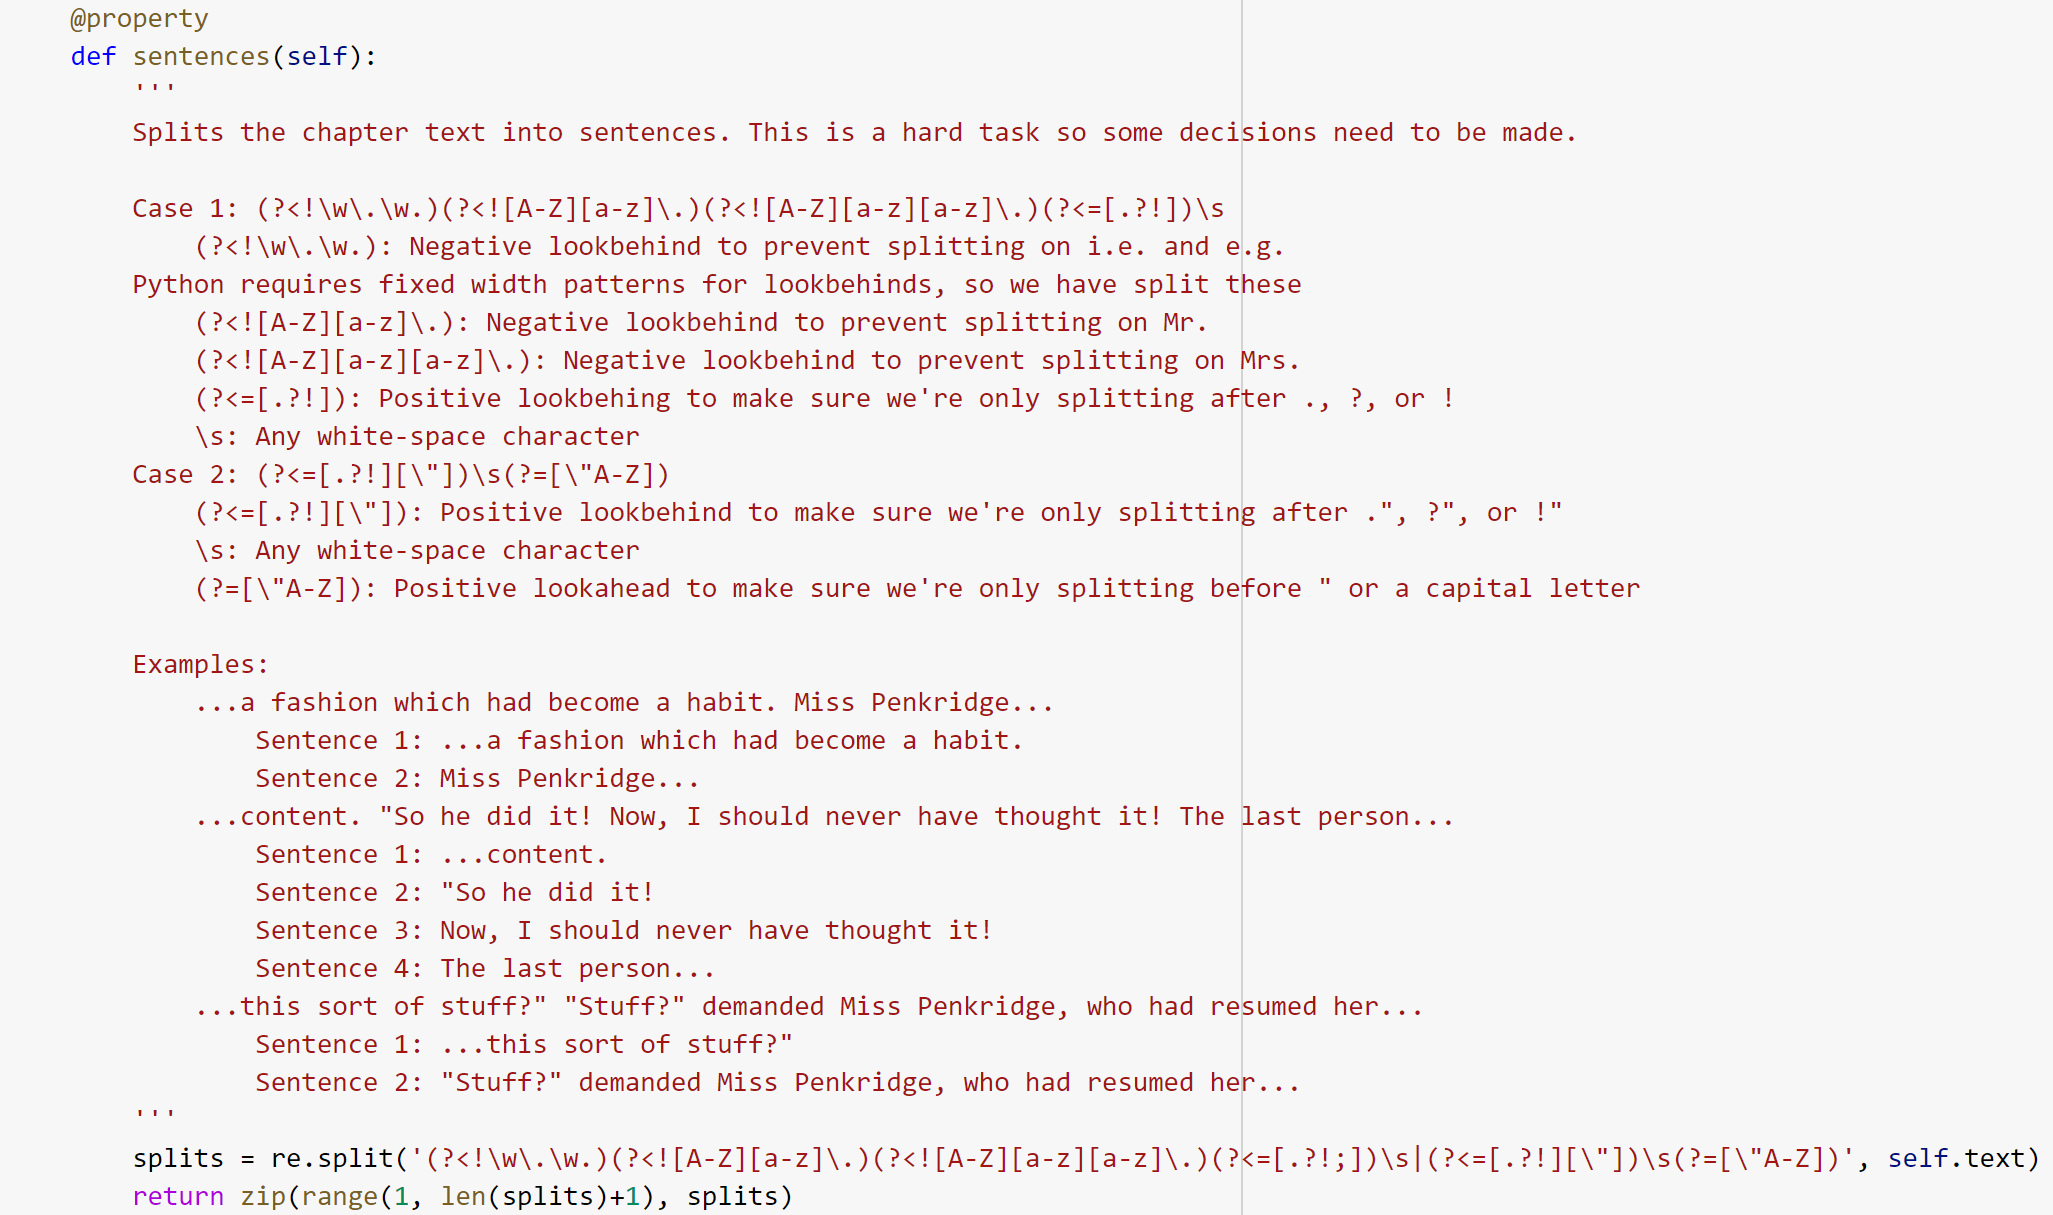
\includegraphics[width=\linewidth]{regex.PNG}
  \caption{A short description of each part of the regex, the cases, and examples of how it splits sentences. Included as a screenshot of python code due to lack of time.}
  \label{fig:sentence-regex}
\end{figure}


\end{document}

